\documentclass[11pt]{report}
% \usepackage[utf8]{inputenc} % pictures
\usepackage[titletoc]{appendix} % appendix
\usepackage[cm]{fullpage} % full page 
\usepackage{nopageno} % Disable bottom page #
\usepackage{multicol} % multicolumn 
\usepackage{enumitem} % list items
\usepackage{fancyhdr} % page headers
\usepackage{titlesec} % title format

% Graphics library for displaying pictures
\usepackage{graphicx}
\graphicspath{ {images/} }

\usepackage{tabu} % allows for tables with width control

% Setting the margins
\usepackage[top=.5in, left=1in, bottom=1in, right=1in]{geometry}
 
% bibliography stuff, to compile use
% user@host~$ pdflatex file.tex
% user@host~$ bibtex file.tex 
% user@host~$ pdflatex file.tex
%
\usepackage[backend=bibtex]{biblatex}
\addbibresource{SRS.bib}

% Create clickable table of contents
\usepackage{hyperref}
\hypersetup {colorlinks,
    citecolor=black,
    filecolor=black,
    linkcolor=black,
    urlcolor=black
}

%set font style
\renewcommand\familydefault{\sfdefault}

% Set line spacing
\renewcommand{\baselinestretch}{1}

% Set indent size
\setlength\parindent{0pt}

% column spacing
\setlength\columnsep{4pt}

% Title format
\titleformat{\chapter}{\Huge\bf}{\thechapter}{20px}{\Huge\bf}


\begin{document}
% Begining of title page

{\Huge \textbf{Software Requirements Specification:}}
\vspace{5mm}
\begin{flushright}

    {\huge for}
    \vspace{20mm}

    \textbf{\Huge Vaultron}
    \vspace{20mm}

    {\huge Version $<0.0.1>$}
    \vspace{20mm}

    {\huge Prepared by}
    \vspace{20mm}

    \textbf{\huge Cryptomaniacs}
    \vspace{20mm}
\end{flushright}

\begin{multicols}{3}
    \noindent
    \begin{itemize}
        \item[] {\Large Colton King}
        \item[] {\Large Grant Wade}
        \item[] {\Large Robby Boney}
        \item[] {\Large Rob Wooner}
    \end{itemize}

    \begin{itemize}
        \item[] {\Large 11245746}
        \item[] {\Large 11435949}
        \item[] {\Large 11453444}
        \item[] {\Large 11496643}
    \end{itemize}

    \begin{itemize}
        \item[] {\Large\texttt colton.king@wsu.edu}
        \item[] {\Large\texttt grant.wade@wsu.edu}
        \item[] {\Large\texttt robby.boney@wsu.edu}
        \item[] {\Large\texttt robert.wooner@wsu.edu}
    \end{itemize}
\end{multicols}

\vfill

\begin{flushright}
    \vspace{20mm}
    {\Large \textbf{Date:} Sunday, October 15th, 2017}
\end{flushright}

% Begining of second page
\clearpage


\tableofcontents{}

\chapter{Introduction}
The goal of this project is to create a cryptographically
secure cross platform password manager. The cross platform
compatibility will be achieved using electron and node.js.
This section will describe who the intended audience for the
password manager will be and describe the purpose of the
project in depth.


\section{Document Purpose}
The product we are writing this SRS document for is the cryptographically
secure cross platform password manager Version 0.0.1 (Vaultron). This password manager 
will create strong passwords and encrypt them. It will remember the password 
for the website it is being created for.


\section{Project Scope}
This software is a password manager that creates cryptographically secure 
passwords. It will store the hashed passwords in a json file for safe keeping.
There can be multiple profiles, each one will have a master password of its own 
that will unlock the vault gaining access to the passwords. The master password
will be created by the user so that they can remember it. The password manager 
can however create a good master password that the user can write down to remember.
the master password will not be sent through email or text so that there will
be no chance of it being stolen from a malicious attacker.

Using this password manager allows the user to have strong and secure passwords 
that they will not have to remember. Not needing to remember allows for a strong 
password that has a very little chance of being cracked. The user only needs to sign
in with their master password and copy and paste the desired password from the 
vault into the website, or other password field.


\section{Intended Audience and Document Overview}
Client: The intended audience of this software is anyone that uses the internet 
and currently keeps track of their passwords by hand or lets the browser
keep track of them. This software will offer a safe, secure, and isolated
way to store any passwords. Security is our number one priority, if something
can be secured it will, so we can ensure that no user data can be leaked.

This document will be used as a starting point to overview the
software. It will describe how it can be used, the security behind the
password storage, and what technologies will be used to create the software.
The rest of the document contains all of the specifications for the
software, which includes product functionality, operating environment,
interface design, functional requirements, behavioral requirements, 
security requirements and other product details.


\section{Definitions, Acronyms and Abbreviations}
\textbf{CSS:} Cascading Style Sheets, used to style our electron application

\textbf{Electron:} Cross platform desktop application development environment
using HTML, CSS, and JavaScript

\textbf{Hardened Mode:} A mode within the product that enable encryption of entire
vault for transport

\textbf{HTML:} HyperText Markup Language, used to design our electron application

\textbf{JavaScript:} Programming language used on the web and Electron

\textbf{Vault:} Password storage platform created for this project


\section{Document Conventions}
IEEE formatting requirements were generally followed when writing this document.
Notable conventions include:

\begin{itemize}
    \item All companies, products and programs are mentioned in itallics (i.e. \textit{electron})
    
\end{itemize}


\section{References and Acknowledgments}

    \nocite{*}
    \printbibliography[heading=none]


% END OF INTRODUCTION

\chapter{Overall Description}

\section{Product Perspective}
At the time of design this project is intended to fill a similar
niche in the password storage and serving field that \textit{1Password}
and \textit{LastPass} fill. Thus it is in the same family as
the two products previously mentioned, a system that stores passwords
securely and allows later retrieval. This product will be implemented in
two main parts. One, a desktop application that will serve as the \textit{vault}
storing the passwords, creating the passwords, and allowing later access
to the passwords. The second main part is the browser extensions that
will be used to auto-fill in usernames and passwords into any website
that the user adds to their vault. 

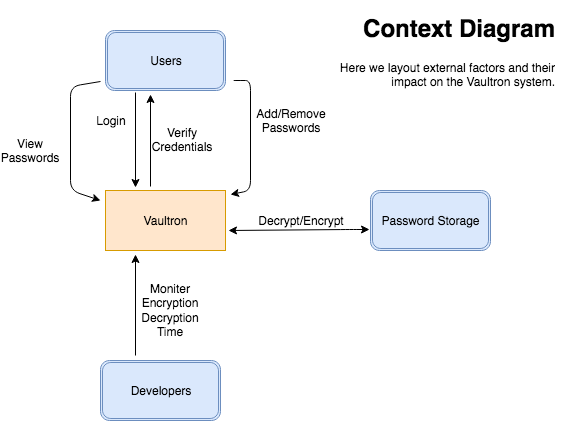
\includegraphics[scale=0.75]{context-diagram}

\section{Product Functionality}

\begin{itemize}
    \item Generate secure passwords (any length or complexity)
    \item Authenticate user to decrypt passwords (required before use)
    \item Generate a \textit{Vault} on first run of software
    \item Allow creation of new entries within the \textit{Vault} (passwords, notes, etc)
    \item Utility to sync users \textit{Vault} between computers (Dropbox, Google Drive, etc)
\end{itemize}

\section{Users and Characteristics}
The users for our software will only need a basic knowledge of how to use 
a computer to use this product. Our users will be a vast majority of people 
that want to only think about one password rather than keeping track of a 
different password for every account they have. All users will be important 
and every user should be confident in the security of their passwords and 
they should also be confident that there will be enough space to have all 
the passwords that they need to store.

Different Types of users:
\begin{itemize}
    \item Basic User
        \begin{itemize}
            \item The user that will only have a few passwords saved in the vault
        \end{itemize}
    \item Power Users
        \begin{itemize}
            \item Users that have over 1000 passwords in the vault
        \end{itemize}
\end{itemize}

\section{Operating Environment}
The environment in which this software will be operating in are all
major operating systems, OS, Windows, Linux. This is accomplished using
\textit{Electron} which allows us to create cross platform binaries
with the same codebase.

\section{Design and Implementation Constraints}
The biggest constraints for this software are time and security considerations.
We need to make sure that our software follows popular, effective, and
accepted security protocols. Given the time frame in which to create this
product and the importance that our password manager successfully encrypts
and protects our passwords, we need to work hard and efficient.

\section{User Documentation}
We will provide a simple help page that will go over how to use and run 
our software. The help page will go over how to create and add a new entry in the 
Vault. How to create a new password. How to delete an old entry. How to update 
an entry.
\section{Assumptions and Dependencies}
Assumptions for \textit{Vaultron} are split into two categories, assumptions
being made about the user and assumptions that are required about components
that are used to create it. 

\subsection{Assumptions about the User}
The assumptions that we are making for the design of this software for the users is
that the users will be using a secure password, and they will not leave
their computers unsecured. On the password side, assumptions have to be
made since we can only put so many constraints on the contents of the
master password. Forcing complexity can result in the user forgetting 
their master password causing them to loose all access to data stored in
\textit{The Vault}. The user leaving their computer unlocked with 
\textit{Vaultron} open could result in someone with access to their computer
copying all the passwords they have stored in \textit{The Vault}. Overall
we have to assume the users will do their best to secure their passwords.

\subsection{Assumptions about the Software}
On the software side we are making the assumption that any components that are
going to be used will not change quickly and without notice. \textit{Vaultron} 
as a whole requires \textit{Node.js} and \textit{Electron} to function, so if 
either were to change it would require a rewrite of the core components of 
this product.


% END OF OVERALL DESCRIPTION

\chapter{Specific Requirements}

\section{External Interface Requirements}

\subsection{User Interfaces}
Our product will have a login window that will have a username text box and password
text box and an enter button. The enter button will be pressed after the password 
and username are inputted. The login window will blur out the rest of the window
behind it.
We will have a minimize, maximize  and exit button in the top left corner. 
we will have tabs along the top that will take you to different password profiles,
like work, play, etc. 
There will be a create password button that will create a pop up that has entries
for a url and a drop down for picking the password profile. 

\subsection{Hardware Interfaces}
Vaultron works on a wide variety of systems with minimal requirement 
mainly due to \textit{Electron's} requirements. The base system specs are as follow:
\\ \\ 
\textbf{Mac}
\begin{itemize}
    \item OS: 64bit
    \item Minimum Version: macOS 10.9
\end{itemize}

\textbf{Windows}
\begin{itemize}
    \item OS: 32bit (x86) or 64bit(amd64)
    \item Minimum Version: Windows 7 and later
\end{itemize}

\textbf{Linux}
\begin{itemize}
    \item OS: 32bit (i686) or 64bit(amd64)
    \item Tested Version: Ubuntu 12.04 
    \item Valid Versions: Ubuntu 12.04 and later, Fedora 21, Debian 8
\end{itemize}


\subsection{Software Interfaces}

\subsection{Communications Interfaces}

\section{Functional Requirements}

\section{Behaviour Requirements}


% END OF SPECIFIC REQUIREMENTS


\chapter{Other Non-Functional Requirements}

\section{Performance Requirements}
The following requirements are based on a system with minimum specs:
\begin{itemize}
    \item Log-in time should not take more than 2 seconds (verifying user)
    \item New entries into the Vault should be less than 1 second before software can be used again
    \item Updating entries should take less than 1 second
    \item Password generation should take less than 1 second
\end{itemize}

\section{Safety and Security Requirements}
Safety and security are the main goals of \textit{Vaultron}, if it is
unable to safely store passwords there is no reason to use it. Therefore
we must abide by some rules. First, any keys created must be generated
from a cryptographically secure random number generator. Our implementation
uses the \textit{Node.js} \texttt{randomBytes()} function to generate
secure random numbers. Secondly, no decrypted passwords will ever be
on any storage device. If a decrypted password was ever stored on a drive
there is a chance that it is recoverable, so passwords will only be 
decrypted on the fly when they are needed and promptly removed from
memory when they are not. Third, all passwords will be stored in their
hashed form within a JSON file. If this file were to be stolen there
would be no direct path to take to decrypt the password hashes because
our implementation will not expose the master decryption key ever.


\section{Software Quality Attributes}


% END OF NONFUNCTIONAL REQUIREMENTS


\chapter{Other Requirements}

\begin{appendices}
    \chapter{Data Dictionary}

    \begin{tabu} to 0.97\textwidth { | X[l] | X[l] | }
        \hline
        Vaultron & our security software  \\
        \hline
        Electron  & javascript wrapper for application development  \\
        \hline
        Node.js  & javascript package for backend related tasks(i.e reading, writing, ect) \\
        \hline
        sqlite  & SQL database being used to store passwords and keys\\
        \hline
        Basic User  & Vaultron user with minimal password requirements \\
        \hline
        Power User  & Vaultron user with extreme password requirements \\
        \hline
        PBKDF2 &  key derivation functions with a sliding computational cost used for encryption. \\
        \hline
    \end{tabu}


    \chapter{Group Log}
\end{appendices}

\end{document}
